\documentclass[11pt]{article}
\usepackage[margin=1in]{geometry}
\usepackage{amsmath,amssymb,amsthm}
\usepackage{graphicx}
\usepackage[hidelinks]{hyperref}
\usepackage{microtype}

\newtheorem{theorem}{Theorem}
\newtheorem{corollary}{Corollary}
\newtheorem{lemma}{Lemma}
\newtheorem{remark}{Remark}

\newcommand{\R}{\mathbb{R}}
\newcommand{\Q}{\mathcal{Q}}
\newcommand{\one}{\mathbf{1}}
\newcommand{\kron}{\mathbin{\otimes}}

\title{Scale, Completeness, and Conjugate Geometry of Landmark Metrics:\\
Classification and Nondegenerate Designs}
\author{Run \texttt{fa\_banach\_001}, lane 12}
\date{2026-07-23}

\begin{document}
\maketitle

\section*{Status}

This packet gives a structural theorem suite for spatial scale covariance,
geodesic completeness, and conjugate geometry of landmark metrics.
\begin{enumerate}
\item For an arbitrary positive-definite landmark cometric \(G(q)\), exact
  dilation covariance of the geodesic flow is equivalent to one power law
  \(G(\lambda q)=\lambda^\alpha G(q)\).
\item A fixed continuous stationary kernel can obey this law only by becoming
  constant and hence degenerate for two or more landmarks.
\item Nondegenerate exactly covariant metrics exist as soon as the bandwidth
  is allowed to follow either the configuration or a global scale coordinate.
  All jointly covariant global-scale kernel families are classified by
  \[
    \kappa_s(x)=s^\alpha\phi(x/s).
  \]
\item Homogeneity itself forces a sharp completeness obstruction: only the
  isometric exponent \(\alpha=2\) can put both total collapse and spatial
  infinity at infinite distance.
\item For every strictly positive-definite matrix profile whose RKHS embeds
  in \(C_b^1\), the adaptive RMS-normalized metric is geodesically complete
  for every \(N,d\) exactly at \(\alpha=2\).  The Gaussian is only one
  instance of this admissible-profile theorem.
\item More generally, an Osgood feature modulus
  \(\omega\), with \(\int_{0}^{1}dt/\omega(t)=\infty\), is sufficient for
  all-\(N\) completeness at \(\alpha=2\).  In fact only the feature gap in
  the instantaneous pair-separation direction needs an Osgood bound.
  For scalar profiles with a
  monotone kernel gap this integral condition is also necessary when
  \(N\ge3\), whereas \(N=2\) is always complete at \(\alpha=2\).  In
  particular, the strict family \(e^{-|z|^\beta}\) is complete for
  \(N\ge3\) exactly at \((\alpha,\beta)=(2,2)\).
\item For every continuous strict stationary matrix profile, the entire
  adaptive two-landmark metric is complete exactly at \(\alpha=2\).  For a
  matrix-valued TRI profile with locally monotone longitudinal gap
  \(\delta_\parallel\), the all-\(N\) criterion is exact: for \(N\ge3\),
  completeness holds exactly when \(\alpha=2\) and
  \(\int_0dr/\sqrt{\delta_\parallel(r)}=\infty\).  The tangential gap does
  not enter.
\item For an arbitrary, possibly irregular non-TRI matrix profile and every
  \(N\), completeness has an exact criterion: quotient by translations and
  dilations and test completeness of an explicit Schur-complement metric on
  the compact normalized pre-shape sphere with its collision diagonals
  deleted.  This is the intrinsic matrix collision-end object for which the
  Osgood and matrix-TRI tests are computable certificates.
\item For every matrix profile, including profiles with an odd skew part,
  the full adaptive two-landmark metric has an explicit center--relative
  block formula.  For even profiles its fixed-center sector is an exact
  Kaluza--Klein metric over \(S^{d-1}\), reducing relative geodesics and
  Jacobi fields to compact magnetic mechanics.
\item For every scalar radial profile, the entire two-landmark manifold at
  \(\alpha=2\) is exactly a scaled product
  \(\mathbb H^{d+1}\times S^{d-1}\).  Its distance, curvature, injectivity
  radius, cut locus, and full ambient conjugate locus are therefore explicit.
\item For an arbitrary matrix-valued TRI profile, the adaptive
  two-landmark fixed-center sector is an exact line--sphere product with
  independently determined radial and spherical scales.
\end{enumerate}
The exponent \(\alpha=2\) makes dilation an actual isometry, not merely a
homothety preserving geodesics.

The source conclusion of Micheli and Glaun\`es~\cite{MG} is a research
program, not one formal conjecture.  The packet now completes the exact-scale
subprogram, the all-\(N\) completeness problem for the full admissible
adaptive-profile class, and the entire two-landmark ambient geometry for
scalar profiles.  It also gives an exact normalized-shape criterion for
every arbitrary matrix profile, extends completeness to Osgood feature moduli,
settles the exact rough/smooth phase diagram for power-exponential adaptive
profiles, proves universal two-landmark completeness for matrix profiles,
and settles all-\(N\) adaptive completeness for matrix-valued TRI profiles
with a locally monotone longitudinal gap.  Application-optimal kernel
selection and a profile-independent closed formula for the full \(N\ge3\)
conjugate locus remain outside this theorem suite; arbitrary-matrix
completeness is now exactly reduced to a compact collision-end metric, while
scalar and matrix-TRI monotone-gap completeness are explicitly classified.

Several literature corrections are essential.  Niethammer and
Vialard~\cite{NV} already proved a broader nonexistence theorem for
scale-invariant geodesic flow of smooth right-invariant LDDMM metrics.  Thus
the fixed-kernel obstruction is not claimed as a new literature resolution.
Habermann--Preston--Sommer~\cite{HPS} completely characterize geodesic
completeness for fixed scalar radial landmark kernels, and
Micheli--Michor--Mumford~\cite{MMM} developed scalar landmark curvature and
conjugate-point mechanisms.  The candidate new portion is therefore confined
to the homogeneous-cometric classification, the adaptive/global-scale
designs, the admissible-profile completeness theorem, the exact
\(\mathbb H^{d+1}\times S^{d-1}\) two-landmark geometry, the matrix-TRI
relative reductions, the configuration-normalized Osgood criterion and
its directional refinement, the universal matrix two-landmark theorem, the
exact scalar and matrix-TRI completeness criteria, the power-exponential
phase diagrams, the arbitrary-matrix normalized-shape classification, the
general two-landmark block and magnetic reductions, and the tail-decoupling
estimate.

\section*{Source Direction and Prior Result}

For a fixed translation-invariant matrix kernel
\(K(x,y)=\kappa(x-y)\), the source landmark Hamiltonian is
\[
 H(p,q)=\frac12\sum_{a,b=1}^{N}
 p_a^{\mathsf T}\kappa(q^a-q^b)p_b,
 \qquad
 \dot q^a=\sum_{b=1}^{N}\kappa(q^a-q^b)p_b.
\]
The source conclusion observes that all examples contain a length constant,
so their landmark and diffeomorphism dynamics are not scale invariant:

\begin{center}

\includegraphics[width=0.98\linewidth]{figures/open_problem_crop.png}
\end{center}

The bounded follow-up search located the following directly relevant prior
result.  Niethammer--Vialard's Theorem~3.2 (printed as Theorem 32) rules out
scale-invariant geodesic flow for every smooth right-invariant metric on the
diffeomorphism group when the symmetry group contains translations,
rotations, and dilations~\cite{NV}.

\begin{center}
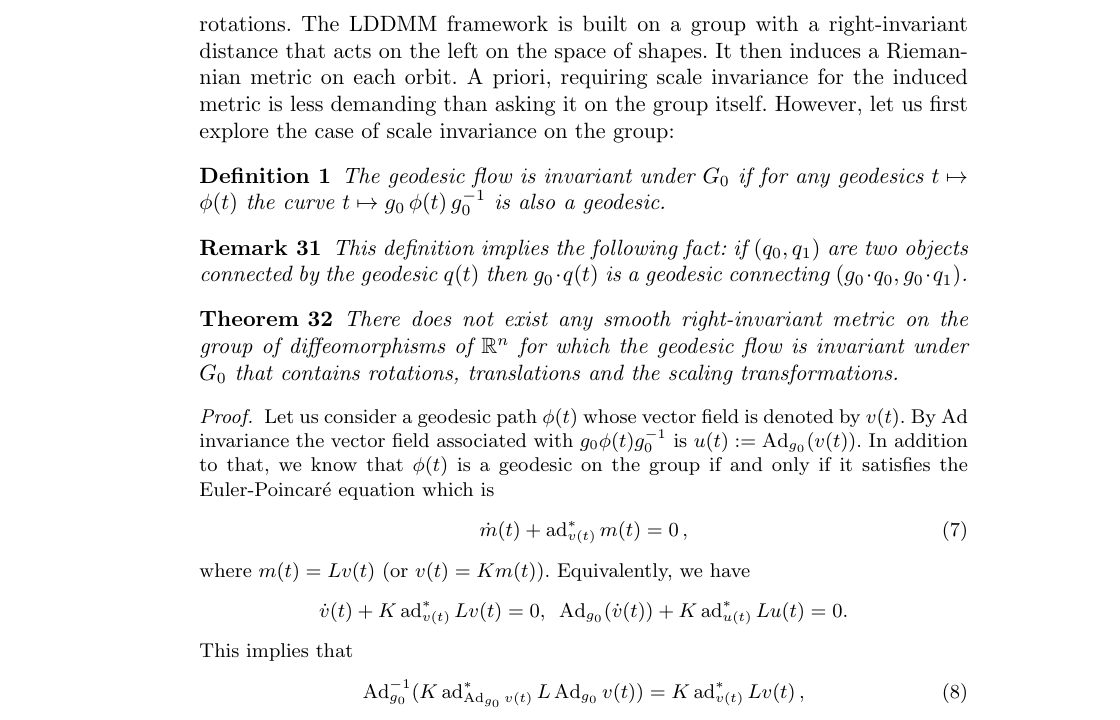
\includegraphics[width=0.91\linewidth]{figures/prior_scale_nonexistence_crop.png}
\end{center}

That theorem is broader at the diffeomorphism-group level.  The elementary
landmark argument below gives a sharp finite-dimensional classification,
including the degenerate boundary, and then identifies two precise ways to
leave the fixed-kernel setting.

\section*{Definitions and Proof Intuition}

Let
\[
 \Q_N=\{q=(q^1,\ldots,q^N)\in(\R^d)^N:q^a\neq q^b\text{ for }a\neq b\}.
\]
A \(C^1\) positive-definite cometric is a map
\(G:\Q_N\to\operatorname{Sym}_{++}(Nd)\).  Its geodesic Hamiltonian is
\begin{equation}
 H(q,p)=\frac12p^{\mathsf T}G(q)p.
 \label{eq:general-H}
\end{equation}
We call its flow \emph{exactly dilation covariant} if for every
\(\lambda>0\) there are \(A_\lambda,C_\lambda>0\), independent of the
solution, such that
\begin{equation}
 Q(t)=\lambda q(C_\lambda t),
 \qquad
 P(t)=A_\lambda p(C_\lambda t)
 \label{eq:covariance}
\end{equation}
is again a solution whenever \((q,p)\) is.

The proof has one central observation.  Since
\(\dot q=G(q)p\), comparing the first Hamilton equation before and after
dilation, for arbitrary \(p\), forces
\[
 G(\lambda q)=h_\lambda G(q).
\]
Composition of dilations makes \(h\) a continuous positive multiplicative
character, hence \(h_\lambda=\lambda^\alpha\).  Conversely, differentiating
this homogeneity law gives exactly the scaling needed in the momentum
equation.  Exact scale covariance is therefore equivalent to homogeneity of
the cometric.

A fixed stationary kernel cannot be homogeneous without collapsing at its
diagonal value.  But if its bandwidth is chosen by a homogeneous
configuration scale \(\rho(q)\), the normalized differences
\((q^a-q^b)/\rho(q)\) do not change under dilation.  This immediately produces
nondegenerate homogeneous Gram matrices.  The same idea with an independent
global scale \(s\) yields a sharp classification of all covariant
scale-indexed families.

The completeness proofs use the cometric directly.  A covector such as
\(d\rho\) or the difference map \(q\mapsto q^a-q^b\) has an easily bounded
cometric norm.  The pair bound is exactly the squared norm of a difference of
RKHS feature maps, so ordinary \(C_b^1\)-admissibility supplies the needed
quadratic estimate for every matrix-valued profile.  Dual Cauchy--Schwarz
then turns these bounds into logarithmic lower bounds on the length required
for total collapse, escape, or a pair collision.

The logarithm is not essential.  If the feature difference has any
nondecreasing modulus \(\omega\), the same argument controls the variation
of the Osgood coordinate \(\int dt/\omega(t)\).  Divergence of that integral
still makes every collision infinitely far away.  Conversely, for a rough
power-exponential profile and \(N\ge3\), let two landmarks collide
symmetrically while the others remain fixed.  In the antisymmetric feature
direction the Gram matrix has a Schur complement
\(S(\varepsilon)\sim C\varepsilon^\beta\); coupling to all noncolliding
features is only \(O(\varepsilon^2)\).  The path speed is therefore
asymptotic to \(C\varepsilon^{-\beta/2}\), which is integrable exactly when
\(\beta<2\).  This produces a finite-length collision and explains the
sharp threshold.

For a matrix profile, controlling the whole feature-gap operator is stronger
than necessary.  The differential of the distance between a pair is the
covector in its instantaneous separation direction, so only the quadratic
form of the feature gap in that same direction enters.  For a TRI profile
this is exactly twice the longitudinal gap
\(\delta_\parallel=a-k_\parallel\).  Collinear configurations preserve the
longitudinal/transverse splitting, so the scalar Schur argument becomes an
exact necessity proof in the longitudinal sector.  The tangential gap is
irrelevant to collision completeness.

For a completely irregular non-TRI profile, no single radial output
direction diagonalizes all collision modes.  The exact replacement is to
remove the two isometric nuisance actions---translations and positive
dilations.  Every orbit has a unique centered, RMS-one representative on a
compact pre-shape sphere.  Orthogonally minimizing over the translation and
dilation directions gives an explicit Schur-complement quotient metric.
A finite-length landmark collision projects to a finite-length path to a
deleted diagonal, and every such quotient path has a horizontal lift of the
same length.  Thus completeness of the original metric is exactly
completeness of this compact collision-end metric.

For two landmarks normalization freezes the profile at separation two.
For every matrix profile, compactness of the direction sphere makes the
resulting normalized two-point Gram matrix uniformly positive, and the
metric is uniformly equivalent to
\(\mathbb H^{d+1}\times S^{d-1}\); this already proves completeness.  In the
scalar case the center/relative Hamiltonian further diagonalizes, and a
constant rescaling of the center coordinate converts the \((c,r)\)-metric
into the upper-half-space metric on \(\mathbb H^{d+1}\), while the direction
of the relative vector supplies a round \(S^{d-1}\).  Thus the full
conjugate and cut geometry is a product calculation, not a numerical
phenomenon.

Without evenness, a matrix profile can have an odd skew part that couples
center and relative momenta.  A direct canonical block calculation isolates
that coupling.  When the profile is even it disappears, and the
fixed-center relative metric completes the square as a Kaluza--Klein metric
over the direction sphere.  Conservation of logarithmic-scale momentum then
gives an exact magnetic Routh reduction.  The TRI line--sphere product is the
zero-connection, constant-coefficient specialization.

\section*{The General Classification}

\begin{theorem}[Homogeneous cometrics are exactly the dilation-covariant ones]
\label{thm:general}
Let \(G:\Q_N\to\operatorname{Sym}_{++}(Nd)\) be \(C^1\).  The Hamiltonian
flow of~\eqref{eq:general-H} is exactly dilation covariant in the sense
of~\eqref{eq:covariance} if and only if there is \(\alpha\in\R\) such that
\begin{equation}
 G(\lambda q)=\lambda^\alpha G(q)
 \qquad(\lambda>0,\ q\in\Q_N).
 \label{eq:Ghom}
\end{equation}
In that case the admissible rescalings satisfy
\[
 A_\lambda=C_\lambda\lambda^{1-\alpha}.
\]
If \(g=G^{-1}\) is the corresponding Riemannian metric and
\(D_\lambda(q)=\lambda q\), then
\begin{equation}
 D_\lambda^*g=\lambda^{2-\alpha}g.
 \label{eq:homothety}
\end{equation}
Thus every \(\alpha\) gives exact covariance of affinely parametrized
geodesics, while \(\alpha=2\) makes every \(D_\lambda\) an isometry.
\end{theorem}

\begin{proof}
Suppose first that the flow is covariant.  Hamilton's first equation applied
to~\eqref{eq:covariance} gives, at \(t=0\),
\[
 \lambda C_\lambda G(q)p=A_\lambda G(\lambda q)p.
\]
The initial momentum is arbitrary, so
\[
 G(\lambda q)=h_\lambda G(q),
 \qquad h_\lambda:=\frac{\lambda C_\lambda}{A_\lambda}>0.
\]
Applying this identity successively with \(\lambda\) and \(\mu\) and using
that \(G(q)\) is invertible gives
\(h_{\lambda\mu}=h_\lambda h_\mu\).  For any fixed \(q\) and nonzero \(u\),
\[
 h_\lambda=
 \frac{u^{\mathsf T}G(\lambda q)u}{u^{\mathsf T}G(q)u},
\]
so \(h\) is continuous.  The continuous positive multiplicative characters
of \((0,\infty)\) are \(h_\lambda=\lambda^\alpha\).  This proves
\eqref{eq:Ghom} and the displayed relation between \(A_\lambda\) and
\(C_\lambda\).

Conversely, differentiating~\eqref{eq:Ghom} in \(q\) gives
\[
 DG(\lambda q)=\lambda^{\alpha-1}DG(q).
\]
Choose any \(C_\lambda>0\) and put
\(A_\lambda=C_\lambda\lambda^{1-\alpha}\).  The transformed first
Hamilton equation scales by
\[
 A_\lambda\lambda^\alpha=\lambda C_\lambda.
\]
The right side of the transformed momentum equation scales by
\[
 A_\lambda^2\lambda^{\alpha-1}
 =A_\lambda C_\lambda,
\]
which is exactly the factor obtained by differentiating
\(P(t)=A_\lambda p(C_\lambda t)\).  Hence both Hamilton equations hold.

Finally, \(G(\lambda q)=\lambda^\alpha G(q)\) implies
\(g_{\lambda q}=\lambda^{-\alpha}g_q\).  Since
\(dD_\lambda=\lambda I\), pulling back the metric gives
\eqref{eq:homothety}.  A constant-factor homothety preserves the
Levi--Civita connection, hence affinely parametrized geodesics.
\end{proof}

\section*{Why Fixed Stationary Kernels Must Degenerate}

\begin{corollary}[Sharp fixed-kernel obstruction]
\label{cor:fixed}
Let \(K(x,y)=\kappa(x-y)\) be a continuous positive-definite
matrix-valued kernel.  If its \(N\)-landmark block Gram cometric is
nondegenerate for \(N\geq2\), its geodesic flow is not exactly dilation
covariant.  If degeneracy is allowed, exact covariance forces
\(\kappa(x)=\kappa(0)\); conversely every constant positive-semidefinite
matrix kernel is covariant and degenerate.
\end{corollary}

\begin{proof}
In the nondegenerate case, Theorem~\ref{thm:general} gives
\[
 \kappa(\lambda(q^a-q^b))
 =\lambda^\alpha\kappa(q^a-q^b).
\]
The diagonal blocks give
\(\kappa(0)=\lambda^\alpha\kappa(0)\).  A nonzero positive-definite
stationary kernel has \(\kappa(0)\neq0\): the kernel Cauchy--Schwarz
inequality
\[
 |u^{\mathsf T}\kappa(x)v|^2
 \leq
 (u^{\mathsf T}\kappa(0)u)(v^{\mathsf T}\kappa(0)v)
\]
shows that \(\kappa(0)=0\) would imply \(\kappa\equiv0\).
Thus \(\alpha=0\), and continuity as \(\lambda\downarrow0\) gives
\(\kappa(x)=\kappa(0)\).

The same conclusion holds without assuming a nondegenerate Gram matrix.
Indeed, use two landmarks with initial positions \((x,0)\) and momenta
\((0,v)\).  Comparing the first Hamilton equation under
\eqref{eq:covariance} directly gives
\[
 \kappa(\lambda x)=h_\lambda\kappa(x).
\]
Positive definiteness and nonzeroness give \(\kappa(0)\neq0\).  Letting
\(x\to0\) in the displayed identity forces \(h_\lambda=1\), and
continuity again makes \(\kappa\) constant.

The \(N\)-landmark Gram matrix is then
\[
  (\one_N\one_N^{\mathsf T})\kron\kappa(0),
\]
whose rank is at most \(d<Nd\).  Conversely, a constant kernel has
\(\dot p_a=0\) and
\(\dot q^a=\kappa(0)\sum_b p_b\), so
\(Q=\lambda q\), \(P=\lambda p\) is again a solution.
\end{proof}

\begin{remark}
In the source's stronger assumption \(V\hookrightarrow
C_0^1(\R^d,\R^d)\), a constant kernel section belongs to \(C_0^1\) only
when it is zero.  Thus the only fixed exactly covariant kernel in that
class is the zero kernel.
\end{remark}

\section*{A Nondegenerate Adaptive Kernel on Landmark Space}

\begin{theorem}[Configuration-adaptive exact scale covariance]
\label{thm:adaptive}
Let \(\rho:\Q_N\to(0,\infty)\) be \(C^2\) and homogeneous of degree one,
\[
 \rho(\lambda q)=\lambda\rho(q).
\]
Let \(\phi:\R^d\to\R^{d\times d}\) be a \(C^2\) profile for which
\((x,y)\mapsto\phi(x-y)\) is a strictly positive-definite matrix kernel.  For any
\(\alpha\in\R\), define the block cometric
\begin{equation}
 G_\alpha(q)_{ab}
 =\rho(q)^\alpha
 \phi\!\left(\frac{q^a-q^b}{\rho(q)}\right).
 \label{eq:adaptive}
\end{equation}
Then \(G_\alpha(q)\) is positive definite on \(\Q_N\), and its geodesic
flow is exactly dilation covariant.  The induced metric satisfies
\[
 D_\lambda^*g_\alpha=\lambda^{2-\alpha}g_\alpha.
\]
In particular, \(\alpha=2\) gives a nondegenerate scale-invariant
Riemannian metric on landmark space.
\end{theorem}

\begin{proof}
The normalized points \(q^a/\rho(q)\) remain pairwise distinct, so strict
positive definiteness of \(\phi\) makes the block matrix in
\eqref{eq:adaptive} positive definite.  Since
\[
 \frac{\lambda q^a-\lambda q^b}{\rho(\lambda q)}
 =\frac{q^a-q^b}{\rho(q)},
\]
we have
\[
 G_\alpha(\lambda q)=\lambda^\alpha G_\alpha(q).
\]
The conclusion follows from Theorem~\ref{thm:general}.
\end{proof}

\begin{corollary}[Explicit RMS--Gaussian metric]
\label{cor:gaussian}
Let
\[
 \bar q=\frac1N\sum_{a=1}^{N}q^a,\qquad
 \rho(q)=
 \left(\frac1N\sum_{a=1}^{N}|q^a-\bar q|^2\right)^{1/2},
\]
and \(\phi(x)=e^{-|x|^2}I_d\).  Formula~\eqref{eq:adaptive} gives a
smooth, nondegenerate landmark metric invariant under translations,
rotations, and permutations.  At \(\alpha=2\), it is also invariant under
all spatial dilations.
\end{corollary}

\begin{proof}
Pairwise distinct landmarks are not all equal, so \(\rho(q)>0\) on
\(\Q_N\); the displayed \(\rho\) is smooth there and has all the stated
symmetries.  The scalar Gaussian is strictly positive definite.  One direct
proof uses its positive Fourier density:
\[
 \sum_{a,b}c_a^{\mathsf T}c_b\,e^{-|x_a-x_b|^2}
 =C_d\int_{\R^d}e^{-|\xi|^2/4}
 \left|\sum_a e^{i\xi\cdot x_a}c_a\right|^2d\xi.
\]
For distinct \(x_a\), the exponential polynomial on the right cannot vanish
identically unless all \(c_a=0\).  Apply Theorem~\ref{thm:adaptive}.
\end{proof}

\begin{remark}[The exact price of the construction]
The cometric in~\eqref{eq:adaptive} does not arise from one fixed ambient
stationary RKHS kernel: its bandwidth depends on the whole landmark
configuration.  This is precisely the assumption that Corollary~\ref{cor:fixed}
shows must be abandoned.  For each fixed value of \(\rho\), however, the
profile is an ordinary smooth positive-definite kernel.
\end{remark}

\section*{A Dynamical Global Scale and Its Complete Kernel Law}

The adaptive construction can be replaced by an independent global scale
coordinate.  This gives a useful classification rather than just an example.

\begin{theorem}[Classification of global-scale kernel Hamiltonians]
\label{thm:augmented}
Let \((\kappa_s)_{s>0}\) be a jointly \(C^2\), nonzero family of
translation-invariant positive-definite matrix kernels, and let
\(b:(0,\infty)\to(0,\infty)\) be \(C^1\).  On the augmented phase space
with scale \(s\) and conjugate momentum \(\pi\), consider
\begin{equation}
 \mathcal H(q,s;p,\pi)
 =\frac12\sum_{a,b}p_a^{\mathsf T}
 \kappa_s(q^a-q^b)p_b+\frac12b(s)\pi^2.
 \label{eq:augH}
\end{equation}
Say that the flow is jointly dilation covariant if, for every \(\lambda>0\),
there are \(A_\lambda,C_\lambda>0\) such that every solution maps to
\[
 Q(t)=\lambda q(C_\lambda t),\quad
 S(t)=\lambda s(C_\lambda t),\quad
 P(t)=A_\lambda p(C_\lambda t),\quad
 \Pi(t)=A_\lambda\pi(C_\lambda t).
\]
This holds if and only if there are \(\alpha\in\R\), \(\beta>0\), and a
positive-definite profile \(\phi\) such that
\begin{equation}
 \boxed{\quad
 \kappa_s(x)=s^\alpha\phi(x/s),
 \qquad b(s)=\beta s^\alpha.
 \quad}
 \label{eq:powerprofile}
\end{equation}
Then \(A_\lambda=C_\lambda\lambda^{1-\alpha}\).  If \(\phi\) is strictly
positive definite, \(\mathcal H\) is a nondegenerate cometric on
\(\Q_N\times(0,\infty)\), and the augmented metric obeys
\[
 D_\lambda^*g=\lambda^{2-\alpha}g,
 \qquad D_\lambda(q,s)=(\lambda q,\lambda s).
\]
\end{theorem}

\begin{proof}
For necessity, use two landmarks with positions \((x,0)\) and momenta
\((0,v)\).  Comparing the first \(q\)-equation before and after dilation
gives
\[
 \kappa_{\lambda s}(\lambda x)=h_\lambda\kappa_s(x),
 \qquad h_\lambda=\frac{\lambda C_\lambda}{A_\lambda}.
\]
The scale equation is \(\dot s=b(s)\pi\).  Its transformed version gives
\[
 b(\lambda s)=h_\lambda b(s).
\]
Since \(b>0\), composition implies
\(h_{\lambda\mu}=h_\lambda h_\mu\), and
\(h_\lambda=b(\lambda)/b(1)\) is continuous.  Hence
\(h_\lambda=\lambda^\alpha\).  Taking \(s=1\), then rescaling by \(s\),
yields~\eqref{eq:powerprofile} with
\(\phi=\kappa_1\) and \(\beta=b(1)\).

For sufficiency, joint homogeneity and differentiation give
\[
\begin{aligned}
 \kappa_{\lambda s}(\lambda x)&=\lambda^\alpha\kappa_s(x),\\
 D_x\kappa_{\lambda s}(\lambda x)
 &=\lambda^{\alpha-1}D_x\kappa_s(x),\\
 \partial_s\kappa_{\lambda s}(\lambda x)
 &=\lambda^{\alpha-1}\partial_s\kappa_s(x),
\end{aligned}
\]
and \(b'(\lambda s)=\lambda^{\alpha-1}b'(s)\).
With \(A_\lambda=C_\lambda\lambda^{1-\alpha}\), the transformed
\(q\)- and \(s\)-equations acquire the factor \(\lambda C_\lambda\);
the transformed \(p\)- and \(\pi\)-equations acquire
\[
 A_\lambda^2\lambda^{\alpha-1}
 =A_\lambda C_\lambda.
\]
These are exactly the factors obtained by differentiating the transformed
variables, proving all four Hamilton equations.

The augmented cometric matrix is
\(\operatorname{diag}(G_s(q),b(s))\), which is positive definite when
\(\phi\) is strictly positive definite.  It scales by
\(\lambda^\alpha\); inversion and \(dD_\lambda=\lambda I\) give the
metric homothety law.
\end{proof}

\begin{corollary}[Frozen-scale family]
For a family~\eqref{eq:powerprofile} with \(s\) treated as an external
parameter, every trajectory for \(s\) maps to a trajectory for
\(\lambda s\) by
\[
 Q(t)=\lambda q(t),\qquad
 P(t)=\lambda^{1-\alpha}p(t).
\]
Thus a scale family restores exact covariance without making the scale
dynamical.
\end{corollary}

\section*{Completeness Selects the Isometric Exponent}

The covariance classification has an immediate global consequence that is
independent of any kernel ansatz.

\begin{theorem}[Radial completeness obstruction]
\label{thm:radial}
Let \(G\) be a positive-definite cometric on a dilation cone and suppose
\(G(rq)=r^\alpha G(q)\).  If the Riemannian metric \(g=G^{-1}\) is
geodesically complete, then \(\alpha=2\).
More precisely, \(\alpha<2\) puts the cone apex at finite distance along every
dilation ray, whereas \(\alpha>2\) puts spatial infinity at finite distance.
\end{theorem}

\begin{proof}
Fix \(u\) in the cone and use the curve \(q(r)=ru\).  Homogeneity gives
\(g_{ru}=r^{-\alpha}g_u\), so its length on an interval \((a,b)\) is
\[
 \sqrt{u^{\mathsf T}g_u u}\int_a^b r^{-\alpha/2}\,dr.
\]
The integral is finite at zero exactly when \(\alpha<2\), and finite at
infinity exactly when \(\alpha>2\).  Either finite-length exit makes the
metric, hence by Hopf--Rinow the geodesic flow, incomplete.
\end{proof}

The converse is false for an arbitrary degree-two cometric because a shape
collision at fixed scale can still be finitely far away.  It becomes true
for the entire adaptive class generated by an admissible stationary RKHS
profile.

\begin{theorem}[Sharp completeness for admissible adaptive profiles]
\label{thm:adaptivecomplete}
Let \(\Phi:\R^d\to\R^{d\times d}\) be \(C^2\), and suppose
\((x,y)\mapsto\Phi(x-y)\) is a strictly positive-definite matrix kernel.
Assume that for some \(L>0\),
\begin{equation}
 0\preccurlyeq
 2\Phi(0)-\Phi(z)-\Phi(-z)
 \preccurlyeq L^2|z|^2I_d
 \qquad(z\in\R^d).
 \label{eq:featureLip}
\end{equation}
For \(N\ge2\), put
\[
 \rho(q)^2=\frac1N\sum_a|q^a-\bar q|^2,
 \qquad
 G^{(\alpha)}(q)_{ab}
 =\rho(q)^\alpha
 \Phi\left(\frac{q^a-q^b}{\rho(q)}\right).
\]
On every connected component of \(\Q_N\), the induced Riemannian metric is
geodesically complete if and only if \(\alpha=2\).

Condition~\eqref{eq:featureLip} holds in particular when \(\Phi\) is the
profile of a stationary vector-valued RKHS \(V\) continuously embedded in
\(C_b^1(\R^d,\R^d)\).
\end{theorem}

\begin{proof}
Strict positive definiteness makes \(G^{(\alpha)}(q)\) positive definite:
the normalized landmarks remain pairwise distinct.  For \(\alpha\ne2\),
Theorem~\ref{thm:radial} supplies a finite-length dilation ray.  It remains
to prove completeness for \(\alpha=2\); write \(G=G^{(2)}\) and
\(T=\operatorname{tr}\Phi(0)\).

For a tangent vector \(v\) and covector \(\ell\), use
\[
 |v|_g^2=v^{\mathsf T}G^{-1}v,
 \qquad |\ell|_G^2=\ell G\ell^{\mathsf T},
 \qquad |\ell(v)|\le |\ell|_G|v|_g.
\]
The normalized block Gram matrix is positive semidefinite and has trace
\(NT\).  Hence
\begin{equation}
 \|G(q)\|_{\rm op}\le NT\rho(q)^2.
 \label{eq:Gop}
\end{equation}
Moreover
\[
 \nabla_{q^a}\rho=\frac{q^a-\bar q}{N\rho},
 \qquad |\nabla\rho|^2=\frac1N.
\]
Equation~\eqref{eq:Gop} gives
\begin{equation}
 |d\rho|_G^2\le T\rho^2,
 \qquad
 \left|\frac d{dt}\log\rho\right|
 \le\sqrt T\,|\dot q|_g.
 \label{eq:rhobound}
\end{equation}
Thus both total collapse and scale escape require infinite length.

For a pair \(a\ne b\), let \(L_{ab}q=q^a-q^b\) and
\(r_{ab}=|q^a-q^b|\).  Direct block subtraction and
\eqref{eq:featureLip} give
\[
\begin{aligned}
 L_{ab}GL_{ab}^{\mathsf T}
 &=\rho^2\left[
 2\Phi(0)-\Phi\left(\frac{q^a-q^b}{\rho}\right)
 -\Phi\left(\frac{q^b-q^a}{\rho}\right)\right]\\
 &\preccurlyeq L^2r_{ab}^2I_d.
\end{aligned}
\]
Applying dual Cauchy--Schwarz to \(dr_{ab}\) yields
\begin{equation}
 \left|\frac d{dt}\log r_{ab}\right|
 \le L|\dot q|_g.
 \label{eq:pairbound}
\end{equation}
Every pair collision is therefore infinitely far away.

A finite-length curve has \(\rho\) bounded above by
\eqref{eq:rhobound}.  Equation~\eqref{eq:Gop} implies
\[
 |\dot q|_{\rm Eucl}
 \le\sqrt{NT}\,\rho|\dot q|_g,
\]
so the curve is Euclidean Cauchy.  It has a finite Euclidean limit, and
\eqref{eq:pairbound} keeps every limiting pair separation positive.  The
limit lies in \(\Q_N\).  This finite-length escape criterion proves metric
completeness, and Hopf--Rinow gives geodesic completeness.

Finally let \(F_xu=K(\,\cdot\,,x)u\) be the feature map of the stationary
RKHS.  The reproducing identity gives
\[
 \|F_xu-F_yu\|_V^2
 =u^{\mathsf T}
 [2\Phi(0)-\Phi(x-y)-\Phi(y-x)]u.
\]
If \(\|v\|_{C_b^1}\le L\|v\|_V\), then
\[
\begin{aligned}
 \|F_xu-F_yu\|_V
 &=\sup_{\|v\|_V=1}|u^{\mathsf T}(v(x)-v(y))|\\
 &\le L|u|\,|x-y|,
\end{aligned}
\]
which is~\eqref{eq:featureLip}.
\end{proof}

\begin{corollary}[Adaptive RMS--Gaussian family]
For
\[
 \Phi(z)=e^{-|z|^2}I_d,
\]
the adaptive family in Theorem~\ref{thm:adaptivecomplete} is complete for
every \(N,d\) exactly at \(\alpha=2\).
\end{corollary}

\begin{proof}
Here
\[
 2\Phi(0)-\Phi(z)-\Phi(-z)
 =2(1-e^{-|z|^2})I_d\preccurlyeq2|z|^2I_d.
\]
\end{proof}

\begin{theorem}[Osgood feature-modulus completeness]
\label{thm:osgood}
Let \(\Phi:\R^d\to\R^{d\times d}\) be continuous, \(C^2\) away from
the origin, and suppose \((x,y)\mapsto\Phi(x-y)\) is a strictly
positive-definite matrix kernel.  Suppose there is a positive
nondecreasing function \(\omega:(0,\infty)\to(0,\infty)\) such that
\begin{equation}
 0\preccurlyeq
 2\Phi(0)-\Phi(z)-\Phi(-z)
 \preccurlyeq \omega(|z|)^2I_d
 \quad(z\ne0),
 \qquad
 \int_0^1\frac{dt}{\omega(t)}=\infty.
 \label{eq:osgood}
\end{equation}
Then, for every \(N\ge2\), the RMS-normalized adaptive family in
Theorem~\ref{thm:adaptivecomplete} is geodesically complete on every
component of \(\Q_N\) if and only if \(\alpha=2\).
\end{theorem}

\begin{proof}
Only sufficiency at \(\alpha=2\) is new.  The trace argument does not use
regularity at the origin, so \eqref{eq:Gop} and \eqref{eq:rhobound} remain
valid.  Consequently, along a curve of finite total length there are
constants \(0<m\le M<\infty\) such that
\[
 m\le\rho(q(t))\le M.
\]
For \(r_{ab}=|q^a-q^b|\), direct block subtraction and
\eqref{eq:osgood} give
\[
 L_{ab}GL_{ab}^{\mathsf T}
 \preccurlyeq
 \rho^2\omega(r_{ab}/\rho)^2I_d.
\]
Dual Cauchy--Schwarz and monotonicity of \(\omega\) therefore imply
\begin{equation}
 |\dot r_{ab}|
 \le \rho\omega(r_{ab}/\rho)|\dot q|_g
 \le M\omega(r_{ab}/m)|\dot q|_g.
 \label{eq:osgoodpair}
\end{equation}
If \(r_{ab}\) approached zero, the change of variable
\[
 \Psi(s)=\int_s^{s_0}\frac{du}{M\omega(u/m)}
\]
would tend to infinity by~\eqref{eq:osgood}, whereas
\eqref{eq:osgoodpair} gives
\(|\frac d{dt}\Psi(r_{ab}(t))|\le|\dot q|_g\).  This is impossible
for a finite-length curve.  Thus every pair separation stays positive.
The operator estimate~\eqref{eq:Gop} again makes the curve Euclidean
Cauchy, with a finite, pairwise-distinct limit.  Metric completeness and
Hopf--Rinow finish the proof.  Necessity of \(\alpha=2\) is
Theorem~\ref{thm:radial}.
\end{proof}

\begin{remark}[The Osgood extension is genuine]
For \(0<c\le2\), the local modulus
\[
 \omega(t)=t(1-\log t)^{c/2}\qquad(0<t\ll1)
\]
satisfies \(\int_0dt/\omega(t)=\infty\), but
\(\omega(t)/t\to\infty\); hence it is not covered by the quadratic
feature estimate~\eqref{eq:featureLip}.  Habermann--Preston--Sommer
\cite{HPS} use precisely the scalar kernel gap
\(\varphi(0)-\varphi(t)=t^2(1-\log t)^c\), \(1<c\le2\), in their
fixed-kernel completeness examples.  Whenever such a profile is used in the
configuration-normalized construction, Theorem~\ref{thm:osgood} supplies
adaptive completeness as well.
\end{remark}

\begin{theorem}[Directional Osgood completeness]
\label{thm:directionalosgood}
Let \(\Phi\) satisfy the continuity, off-origin \(C^2\), and strict
positive-definiteness hypotheses of Theorem~\ref{thm:osgood}.  Suppose there
is a positive nondecreasing \(\omega\) such that, for every \(t>0\) and unit
vector \(e\),
\begin{equation}
 e^{\mathsf T}
 \bigl[2\Phi(0)-\Phi(te)-\Phi(-te)\bigr]e
 \le\omega(t)^2,
 \qquad
 \int_0^1\frac{dt}{\omega(t)}=\infty.
 \label{eq:directionalosgood}
\end{equation}
Then, for every \(N\ge2\), the RMS-normalized adaptive family is
geodesically complete exactly when \(\alpha=2\).
\end{theorem}

\begin{proof}
Only sufficiency is new.  Let
\(z=q^a-q^b=r e\), where \(r>0\) and \(|e|=1\), and let \(L_{ab}\)
be the pair-difference map.  Direct block subtraction gives
\[
 L_{ab}GL_{ab}^{\mathsf T}
 =\rho^2
 \left[
 2\Phi(0)-\Phi\left(\frac r\rho e\right)
             -\Phi\left(-\frac r\rho e\right)
 \right].
\]
Since \(dr=e^{\mathsf T}L_{ab}\), its squared cometric norm satisfies
\[
 |dr|_G^2
 =e^{\mathsf T}L_{ab}GL_{ab}^{\mathsf T}e
 \le\rho^2\omega(r/\rho)^2.
\]
Along a finite-length curve the scale estimate~\eqref{eq:rhobound} gives
\(0<m\le\rho\le M<\infty\).  Dual Cauchy--Schwarz therefore yields
\[
 |\dot r|
 \le M\omega(r/m)|\dot q|_g.
\]
The Osgood-coordinate argument in Theorem~\ref{thm:osgood} now excludes
every pair collision.  The trace estimate~\eqref{eq:Gop} makes the curve
Euclidean Cauchy, so its limit lies in \(\Q_N\).  Hopf--Rinow proves
completeness.  Theorem~\ref{thm:radial} excludes \(\alpha\ne2\).
\end{proof}

\begin{theorem}[Universal adaptive two-landmark matrix completeness]
\label{thm:matrixNtwo}
Let \(\Phi:\R^d\to\R^{d\times d}\) be continuous and \(C^2\) away from the
origin, and suppose its stationary matrix kernel is strictly positive
definite.  For \(N=2\), the RMS-normalized adaptive metric is geodesically
complete exactly when \(\alpha=2\).
\end{theorem}

\begin{proof}
Necessity is Theorem~\ref{thm:radial}.  Let \(\alpha=2\), and write
\[
 c=\frac{q^1+q^2}{2},\qquad
 q^1-q^2=r e,\qquad r>0,\quad |e|=1.
\]
Then \(\rho=r/2\), and the normalized block Gram matrix is
\[
 K(e)=
 \begin{pmatrix}
  \Phi(0)&\Phi(2e)\\
  \Phi(-2e)&\Phi(0)
 \end{pmatrix}.
\]
It is positive definite for every \(e\).  Continuity and compactness of
\(S^{d-1}\) give constants \(0<m_0\le M_0<\infty\) with
\[
 m_0I_{2d}\preccurlyeq K(e)\preccurlyeq M_0I_{2d}
 \qquad(e\in S^{d-1}).
\]
Moreover
\[
 |dq|_{\rm Eucl}^2
 =2|dc|^2+\frac12\bigl(dr^2+r^2|de|^2\bigr).
\]
Since \(G=\rho^2K(e)\), the adaptive metric is uniformly equivalent to
\begin{equation}
 \frac{|dc|^2+dr^2}{r^2}+|de|^2,
 \label{eq:matrixNtwomodel}
\end{equation}
the product of an upper-half-space hyperbolic metric with the round sphere.
This model is complete, and uniform equivalence preserves metric
completeness.  Hopf--Rinow finishes the proof.
\end{proof}

\begin{theorem}[Exact scalar adaptive completeness criterion]
\label{thm:scalarcriterion}
Let \(\Phi(z)=\varphi(|z|)I_d\) be a continuous strictly
positive-definite scalar radial profile, \(C^2\) away from the origin.
Put
\[
 \delta(r)=\varphi(0)-\varphi(r),
\]
and suppose \(\delta\) is nondecreasing on some interval \((0,r_0)\).
For the RMS-normalized adaptive power family:
\begin{enumerate}
\item if \(N=2\), the metric is geodesically complete exactly when
  \(\alpha=2\);
\item if \(N\ge3\), the metric is geodesically complete exactly when
  \begin{equation}
   \alpha=2
   \quad\text{and}\quad
   \int_0^{r_0}\frac{dr}{\sqrt{\delta(r)}}=\infty.
   \label{eq:scalarcriterion}
  \end{equation}
\end{enumerate}
When the integral is finite, incompleteness is witnessed by a
finite-length curve along which exactly two landmarks collide while
\(\rho\) stays bounded away from zero.
\end{theorem}

\begin{proof}
The \(N=2\) statement is Theorem~\ref{thm:matrixNtwo}.  Let \(N\ge3\).
If the integral diverges,
define
\[
 \omega(t)^2=2\sup_{0<s\le t}\delta(s).
\]
Two-point strict positive definiteness gives \(\delta(s)>0\) for \(s>0\),
and the kernel Cauchy--Schwarz inequality bounds \(\delta\), so \(\omega\)
is positive and nondecreasing.  Near zero,
\(\omega(t)^2=2\delta(t)\), and the scalar feature gap is
\[
 2\Phi(0)-\Phi(z)-\Phi(-z)=2\delta(|z|)I_d
 \preccurlyeq\omega(|z|)^2I_d.
\]
Theorem~\ref{thm:osgood} proves completeness at \(\alpha=2\);
Theorem~\ref{thm:radial} excludes every other exponent.

Conversely, suppose the integral in~\eqref{eq:scalarcriterion} is finite.
Monotonicity forces
\begin{equation}
 \frac{\delta(r)}{r^2}\longrightarrow\infty
 \qquad(r\downarrow0).
 \label{eq:gapsuperquadratic}
\end{equation}
Indeed, otherwise there are \(C<\infty\) and a sequence
\(r_j\downarrow0\), chosen with \(r_{j+1}<r_j/2\), such that
\(\delta(r_j)\le Cr_j^2\).  On every disjoint interval
\([r_j/2,r_j]\), monotonicity would give
\[
 \int_{r_j/2}^{r_j}\frac{dr}{\sqrt{\delta(r)}}
 \ge\frac1{2\sqrt C},
\]
contradicting finiteness of the integral.

Fix a unit vector \(e\), choose mutually distinct nonzero sites
\(x_3,\ldots,x_N\), and consider
\begin{equation}
 q^1(\varepsilon)=-\varepsilon e,\qquad
 q^2(\varepsilon)= \varepsilon e,\qquad
 q^j(\varepsilon)=x_j\quad(j\ge3).
 \label{eq:collisionpath}
\end{equation}
The mean is independent of \(\varepsilon\), while
\[
 \rho(\varepsilon)^2=\rho(0)^2+\frac{2}{N}\varepsilon^2,
 \qquad \rho(0)>0.
\]
Set \(t_\varepsilon=2\varepsilon/\rho(\varepsilon)\), and let
\(K_\varepsilon\) be the normalized scalar Gram matrix.  In the basis
whose first vector is
\[
 u=\frac{1}{\sqrt2}(1,-1,0,\ldots,0),
\]
write
\[
 K_\varepsilon=
 \begin{pmatrix}
  a_\varepsilon&b_\varepsilon^{\mathsf T}\\
  b_\varepsilon&C_\varepsilon
 \end{pmatrix},
 \qquad a_\varepsilon=\delta(t_\varepsilon).
\]
At \(\varepsilon=0\), \(C_0\) is the weighted Gram matrix of the
\(N-1\) distinct normalized sites
\[
 0,\quad x_3/\rho(0),\quad\ldots,\quad x_N/\rho(0),
\]
and hence is positive definite.
Smoothness at their nonzero separations yields
\[
 b_\varepsilon=O(\varepsilon),\qquad
 C_\varepsilon^{-1}=O(1).
\]
Since \(t_\varepsilon\sim2\varepsilon/\rho(0)\),
\eqref{eq:gapsuperquadratic} gives
\(\varepsilon^2=o(a_\varepsilon)\).  Thus the Schur complement satisfies
\begin{equation}
 S_\varepsilon
 =a_\varepsilon-
 b_\varepsilon^{\mathsf T}C_\varepsilon^{-1}b_\varepsilon
 =a_\varepsilon(1+o(1)).
 \label{eq:schurasymptotic}
\end{equation}

The path velocity is \(-\sqrt2\,u\otimes e\), and exact block inversion
gives
\[
 |\dot q(\varepsilon)|_g^2
 =\frac{2}{\rho(\varepsilon)^2S_\varepsilon}.
\]
The map \(\varepsilon\mapsto t_\varepsilon\) is a \(C^1\)
diffeomorphism near zero with derivative bounded above and below.
Consequently the remaining path length is bounded by a constant times
\[
 \int_0^{\varepsilon_0}
 \frac{d\varepsilon}{\sqrt{\delta(t_\varepsilon)}}
 \asymp
 \int_0^{t_{\varepsilon_0}}\frac{dt}{\sqrt{\delta(t)}}<\infty.
\]
Its limit has \(q^1=q^2\), so the metric is incomplete.
\end{proof}

\begin{corollary}[Exact power-exponential phase diagram]
\label{thm:stablephase}
For \(0<\beta\le2\), let
\[
 \Phi_\beta(z)=e^{-|z|^\beta}I_d.
\]
The corresponding RMS-normalized adaptive metric is geodesically complete
exactly for
\[
\begin{array}{c|c}
 \text{number of landmarks}&
 \text{complete parameters}\\ \hline
 N=2&\alpha=2,\quad 0<\beta\le2,\\
 N\ge3&\alpha=2,\quad \beta=2.
\end{array}
\]
\end{corollary}

\begin{proof}
Schoenberg's theorem~\cite{Schoenberg} gives strict positive definiteness:
\(t\mapsto e^{-t^{\beta/2}}\) is a positive mixture of Gaussian profiles
with positive scales, each of which is strict.  Moreover
\(\delta(r)=1-e^{-r^\beta}\) is increasing and
\(\delta(r)\sim r^\beta\).  Hence
\(\int_0dr/\sqrt{\delta(r)}\) diverges exactly when \(\beta\ge2\).
Apply Theorem~\ref{thm:scalarcriterion}.
\end{proof}

\begin{theorem}[Exact matrix-TRI adaptive completeness criterion]
\label{thm:matrixtricriterion}
Let \(\Phi\) be a continuous strictly positive-definite TRI matrix profile,
\(C^2\) away from the origin, and write
\[
 \Phi(0)=aI_d,\qquad
 \Phi(re)=k_\parallel(r)P_e+k_\perp(r)P_e^\perp
 \quad(r>0,\ |e|=1).
\]
Put
\[
 \delta_\parallel(r)=a-k_\parallel(r),
\]
and suppose \(\delta_\parallel\) is nondecreasing on some interval
\((0,r_0)\).  For the RMS-normalized adaptive power family:
\begin{enumerate}
\item if \(N=2\), the metric is geodesically complete exactly when
  \(\alpha=2\);
\item if \(N\ge3\), the metric is geodesically complete exactly when
  \begin{equation}
   \alpha=2
   \quad\text{and}\quad
   \int_0^{r_0}\frac{dr}{\sqrt{\delta_\parallel(r)}}=\infty.
   \label{eq:matrixtricriterion}
  \end{equation}
\end{enumerate}
Thus collision completeness depends only on the longitudinal gap; no
condition on the tangential gap
\(\delta_\perp(r)=a-k_\perp(r)\) is needed.
\end{theorem}

\begin{proof}
The two-landmark statement is Theorem~\ref{thm:matrixNtwo}.  Let \(N\ge3\).
For \(z=te\), the directional feature gap in
\eqref{eq:directionalosgood} is
\[
 e^{\mathsf T}[2\Phi(0)-\Phi(te)-\Phi(-te)]e
 =2\delta_\parallel(t).
\]
If the integral in~\eqref{eq:matrixtricriterion} diverges, take
\[
 \omega(t)^2=2\sup_{0<s\le t}\delta_\parallel(s).
\]
Near zero this is \(2\delta_\parallel(t)\), and
Theorem~\ref{thm:directionalosgood} proves completeness at \(\alpha=2\).
Theorem~\ref{thm:radial} excludes the other exponents.

Conversely, suppose the integral is finite.  The dyadic argument proving
\eqref{eq:gapsuperquadratic} applies verbatim and gives
\[
 \frac{\delta_\parallel(r)}{r^2}\longrightarrow\infty.
\]
Fix a unit vector \(e\), choose distinct nonzero scalars
\(x_3,\ldots,x_N\), and use the collinear path
\[
 q^1=-\varepsilon e,\qquad q^2=\varepsilon e,\qquad
 q^j=x_j e\quad(j\ge3).
\]
All normalized differences are parallel to \(e\), so every Gram block
preserves
\(\R e\oplus e^\perp\).  The collision velocity lies in the longitudinal
sector.  On that sector the normalized Gram matrix is the scalar matrix
\[
 (K_\varepsilon^\parallel)_{ij}
 =k_\parallel\left(
   \frac{|q^i-q^j|}{\rho(\varepsilon)}
  \right).
\]
Strict matrix positive definiteness implies strict positive definiteness of
this scalar Gram matrix: test the original kernel only on coefficients
parallel to \(e\).

In the landmark basis whose first vector is
\(u=(1,-1,0,\ldots,0)/\sqrt2\), write
\[
 K_\varepsilon^\parallel=
 \begin{pmatrix}
  a_\varepsilon&b_\varepsilon^{\mathsf T}\\
  b_\varepsilon&C_\varepsilon
 \end{pmatrix}.
\]
Exactly as in the scalar proof,
\[
 a_\varepsilon
 =\delta_\parallel(2\varepsilon/\rho(\varepsilon)),\qquad
 b_\varepsilon=O(\varepsilon),\qquad
 C_\varepsilon^{-1}=O(1).
\]
The superquadratic ratio makes
\(\varepsilon^2=o(a_\varepsilon)\), hence
\[
 S_\varepsilon^\parallel
 =a_\varepsilon-
 b_\varepsilon^{\mathsf T}C_\varepsilon^{-1}b_\varepsilon
 =a_\varepsilon(1+o(1)).
\]
Exact block inversion in the invariant longitudinal sector gives
\[
 |\dot q(\varepsilon)|_g^2
 =\frac{2}{
 \rho(\varepsilon)^2S_\varepsilon^\parallel}.
\]
The same \(C^1\) change of variable
\(t=2\varepsilon/\rho(\varepsilon)\) as in
Theorem~\ref{thm:scalarcriterion} shows that the collision path has finite
length.  Its limit has \(q^1=q^2\), proving incompleteness.
\end{proof}

\begin{corollary}[Genuinely matrix-valued power-exponential phase diagram]
\label{cor:matrixstablephase}
Let \(d\ge2\), \(\eta>0\), \(0<\beta\le2\), and
\[
 \Phi_{\beta,\eta}(z)
 =e^{-|z|^\beta}I_d
  +\eta\left[-D^2e^{-|z|^2}\right].
\]
This is a strict, genuinely matrix-valued TRI kernel.  Its adaptive metric
is complete exactly for
\[
\begin{array}{c|c}
 \text{number of landmarks}&\text{complete parameters}\\ \hline
 N=2&\alpha=2,\quad 0<\beta\le2,\\
 N\ge3&\alpha=2,\quad \beta=2.
\end{array}
\]
\end{corollary}

\begin{proof}
Schoenberg's theorem~\cite{Schoenberg} gives strict positive definiteness of the first
summand.  The Fourier transform of the second is a positive scalar multiple
of
\(\xi\xi^{\mathsf T}e^{-|\xi|^2/4}\), so it is a positive-semidefinite
matrix kernel.  Their sum is strict, and for \(\eta>0\) it is not a scalar
multiple of \(I_d\).

Along \(z=re\), its longitudinal coefficient is
\[
 k_\parallel(r)
 =e^{-r^\beta}+\eta(2-4r^2)e^{-r^2},
\]
while \(\Phi_{\beta,\eta}(0)=(1+2\eta)I_d\).  Hence
\[
 \delta_\parallel(r)
 =1-e^{-r^\beta}
  +\eta\left[2-(2-4r^2)e^{-r^2}\right].
\]
This is increasing near zero and is asymptotic to \(r^\beta\) for
\(\beta<2\), and to \((1+6\eta)r^2\) for \(\beta=2\).  Apply
Theorem~\ref{thm:matrixtricriterion}.
\end{proof}

\begin{theorem}[Exact full two-landmark scalar geometry]
\label{thm:scalarproduct}
Let \(\Phi(z)=\varphi(|z|)I_d\) be any continuous strictly
positive-definite scalar radial profile.  For the adaptive construction with
\(N=2\) and \(\alpha=2\), set
\[
 a=\varphi(0),\qquad b=\varphi(2),\qquad
 B=\frac{2}{a-b}.
\]
Write
\[
 c=\frac{q^1+q^2}{2},\qquad
 q^1-q^2=r\omega,\qquad
 x=2\sqrt{\frac{a-b}{a+b}}\,c.
\]
Then \(a\pm b>0\), and the entire two-landmark metric is
\begin{equation}
 \boxed{\quad
 g=B\left[
 \frac{dr^2+|dx|^2}{r^2}+g_{S^{d-1}}
 \right].
 \quad}
 \label{eq:Hsphere}
\end{equation}
Thus each connected component is isometric to the scaled product
\[
 B\left(\mathbb H^{d+1}\times S^{d-1}\right).
\]
For the corresponding adaptive power family, the full two-landmark metric is
complete if and only if \(\alpha=2\).
\end{theorem}

\begin{proof}
Use the canonical variables
\[
 z=q^1-q^2,\quad P=p_1+p_2,\quad
 \pi=\frac{p_1-p_2}{2}.
\]
Since \(\rho=r/2\), the diagonal and off-diagonal cometric blocks are
\(\rho^2aI_d\) and \(\rho^2bI_d\).  The Hamiltonian is
\[
 H=\frac{\rho^2(a+b)}4|P|^2
   +\rho^2(a-b)|\pi|^2.
\]
Strict two-point positive definiteness gives \(a\pm b>0\).  Inverting the
center and relative cometric blocks gives
\[
 g=\frac{8}{r^2(a+b)}|dc|^2
  +\frac{2}{a-b}
   \left(\frac{dr^2}{r^2}+g_{S^{d-1}}\right).
\]
The stated rescaling of \(c\) turns this into~\eqref{eq:Hsphere}; the
first term in brackets is the upper-half-space metric on
\(\mathbb H^{d+1}\).  The product is complete.  All other exponents are
incomplete by Theorem~\ref{thm:radial}.
\end{proof}

\begin{corollary}[Distance, curvature, cut locus, and conjugate locus]
\label{cor:fullgeometry}
Represent a point in Theorem~\ref{thm:scalarproduct} by
\((h,\omega)\), where \(h=(x,r)\in\mathbb H^{d+1}\).  For \(d\ge2\),
\[
\begin{aligned}
 d_g((h_0,\omega_0),(h_1,\omega_1))^2
 &=B\left[d_{\mathbb H}(h_0,h_1)^2+\theta^2\right],\\
 \theta&=\arccos(\omega_0^{\mathsf T}\omega_1),\\
 \cosh d_{\mathbb H}(h_0,h_1)
 &=1+\frac{|x_0-x_1|^2+(r_0-r_1)^2}{2r_0r_1}.
\end{aligned}
\]
Sectional curvature is \(-1/B\) on hyperbolic planes, \(1/B\) on
spherical planes, and zero on mixed planes.  The injectivity radius is
\(\pi\sqrt B\), and the cut locus of \((h_0,\omega_0)\) is
\[
 \mathbb H^{d+1}\times\{-\omega_0\}.
\]

For \(d\ge3\), the exponential is singular exactly at tangent vectors whose
standard-sphere component has length \(m\pi\), \(m=1,2,\ldots\), with
multiplicity \(d-2\).  The first conjugate locus is
\(\mathbb H^{d+1}\times\{-\omega_0\}\), while the set of all conjugate
endpoints is
\[
 \mathbb H^{d+1}\times\{\omega_0,-\omega_0\}.
\]
In particular, a pure angular great circle has its first \emph{ambient}
conjugate point at length \(\pi\sqrt B\), with multiplicity \(d-2\).
For \(d=2\), the circle factor has cut points but no conjugate points, so the
full manifold has no conjugate points.  For \(d=1\), each order component is
a scaled hyperbolic plane.
\end{corollary}

\begin{proof}
All assertions are the standard product consequences of
\eqref{eq:Hsphere}.  Hyperbolic space has no cut or conjugate points.  On
the unit round sphere, the cut point is the antipode and the differential of
the exponential is singular when the tangent length is \(m\pi\), with kernel
dimension \(d-2\).  Multiplying the metric by \(B\) multiplies lengths by
\(\sqrt B\) and curvatures by \(1/B\).
\end{proof}

\begin{corollary}[Adaptive matrix-TRI fixed-center product]
\label{cor:matrixadaptive}
Let \(\Phi\) be a strictly positive-definite TRI matrix profile and write
\[
 \Phi(0)=aI_d,\qquad
 \Phi(2\omega)
 =k_\parallel(2)P_\parallel+k_\perp(2)P_\perp.
\]
Set
\[
 \delta_\parallel=a-k_\parallel(2),\qquad
 \delta_\perp=a-k_\perp(2).
\]
For \(N=2\) and \(\alpha=2\), the fixed-center sector is totally geodesic
and has the exact product metric
\begin{equation}
 g_{\rm rel}
 =\frac{2}{\delta_\parallel}\,ds^2
  +\frac{2}{\delta_\perp}\,g_{S^{d-1}},
 \qquad s=\log|q^1-q^2|.
 \label{eq:adaptiveTRIproduct}
\end{equation}
Its distance, cut locus, and conjugate locus are the corresponding
line--sphere product formulas.  For \(d\ge3\), the first pure-angular sector
conjugate length is
\[
 \pi\sqrt{\frac{2}{\delta_\perp}},
\]
with multiplicity \(d-2\); these sector Jacobi fields are also ambient
Jacobi fields.
\end{corollary}

\begin{proof}
Translation invariance conserves \(P=p_1+p_2\), and the center velocity
vanishes when \(P=0\), so the fixed-center sector is totally geodesic.
The relative cometric is
\[
 2\rho^2[\Phi(0)-\Phi(2\omega)]
 =\frac{r^2}{2}
  [\delta_\parallel P_\parallel+\delta_\perp P_\perp].
\]
Inversion and \(z=r\omega\) give~\eqref{eq:adaptiveTRIproduct}.  The
remaining claims follow from the product exponential and Jacobi equation.
\end{proof}

\section*{Regularity and Generic Two-Landmark TRI Geometry}

For fixed scalar radial kernels, the global completeness question is already
answered.  Bauer--Bruveris--Michor's Theorem~9.8 gives completeness under the
standard \(C_b^1\)-admissibility hypothesis~\cite{BBM}, and
Habermann--Preston--Sommer prove the sharp all-\(N\), all-\(d\) criterion
\[
 \int_0^a\frac{dr}{\sqrt{K(0)-K(r)}}=\infty
\]
for scalar radial kernels smooth away from the origin~\cite{HPS}.  The next
theorem records the matrix-valued two-landmark reduction suggested by the
source.

\begin{theorem}[Matrix-TRI relative reduction]
\label{thm:matrixtri}
Let \(\kappa\) be a continuous, strictly positive-definite, rotation- and
translation-invariant matrix kernel, \(C^2\) away from the origin.  Write
\[
 \kappa(0)=aI_d,
 \qquad
 \kappa(z)=k_\parallel(r)P_\parallel+k_\perp(r)P_\perp,
 \qquad r=|z|,
\]
and set \(\delta_\parallel=a-k_\parallel\),
\(\delta_\perp=a-k_\perp\).  On the two-landmark fixed-center sector,
\begin{equation}
 g_{\rm rel}
 =\frac{dr^2}{2\delta_\parallel(r)}
 +\frac{r^2}{2\delta_\perp(r)}\,g_{S^{d-1}}.
 \label{eq:trimetric}
\end{equation}
It is complete if and only if
\[
 \int_0^\epsilon\frac{dr}{\sqrt{\delta_\parallel(r)}}=\infty.
\]
If
\[
 \frac{ds}{dr}=\frac1{\sqrt{2\delta_\parallel(r)}},
 \qquad
 f(s)=\frac{r}{\sqrt{2\delta_\perp(r)}},
\]
then its radial and tangential sectional curvatures are
\[
 K_{\rm rad}=-\frac{f''(s)}{f(s)},
 \qquad
 K_{\rm tan}=\frac{1-f'(s)^2}{f(s)^2}\quad(d\ge3).
\]
\end{theorem}

\begin{proof}
In the canonical center/relative variables used above, setting \(P=0\)
gives
\[
 H_{\rm rel}
 =\pi^{\mathsf T}(\kappa(0)-\kappa(z))\pi.
\]
The radial and tangential eigenvalues of the relative cometric are therefore
\(2\delta_\parallel\) and \(2\delta_\perp\).  Inversion proves
\eqref{eq:trimetric}.  Any curve changing radius from \(r_0\) to \(r_1\) has
length at least the integral of
\(dr/\sqrt{2\delta_\parallel(r)}\), with equality for a radial curve.
Two-point positive definiteness gives
\(0<\delta_\parallel(r)\le2a\), so Euclidean infinity is always infinitely
far away.  On compact radial annuli the metric is uniformly nondegenerate;
the displayed collision integral is therefore necessary and sufficient for
completeness.  The change to \(s\) turns~\eqref{eq:trimetric} into the warped
product \(ds^2+f(s)^2g_{S^{d-1}}\), whose standard curvature formulas give the
last assertion.
\end{proof}

For a scalar kernel \(\delta_\parallel=\delta_\perp=\delta\), the relative
Gaussian curvature in \(d=2\) is
\[
 K_{\rm rel}(r)
 =\delta(r)\left(\frac{d^2}{dr^2}+\frac1r\frac d{dr}\right)\log\delta(r).
\]
For \(K(r)=e^{-r^2/(2\sigma^2)}\), with
\(t=r^2/(2\sigma^2)\), this becomes
\[
 K_{\rm rel}(r)=\frac{2}{\sigma^2}
 \frac{e^t(1-t)-1}{e^t(e^t-1)}<0.
\]
This intrinsic fixed-center surface is complete and has no conjugate points.
The broader scalar landmark curvature and conjugate-point mechanisms were
already developed by Micheli--Michor--Mumford~\cite{MMM}; this calculation is
included to connect Theorem~\ref{thm:matrixtri} to that literature, not as a
new scalar result.

\section*{What Kernel Tails Control}

\begin{theorem}[Quantitative cluster decoupling]
\label{thm:tails}
Let \(\kappa\) be a stationary \(C^2\) matrix kernel and define
\[
 \eta(R)=\sup_{|x|\ge R}
 \bigl(\|\kappa(x)\|+\|D\kappa(x)\|\bigr).
\]
Partition the landmarks into clusters and let \(X_0\) be the Hamiltonian
system obtained by deleting cross-cluster terms.  On a phase-space region
where \(|p_a|\le P\) and every intercluster separation is at least \(R\),
the full and decoupled vector fields satisfy
\[
 \|F-F_0\|\le C(N,P)\eta(R).
\]
If \(F_0\) has Lipschitz constant \(L\) on that region and both trajectories
remain there through time \(T\), then equal initial data satisfy
\[
 \|X(t)-X_0(t)\|
 \le C(N,P)\eta(R)\frac{e^{Lt}-1}{L},
 \qquad 0\le t\le T,
\]
with the usual interpretation \(t\) when \(L=0\).
\end{theorem}

\begin{proof}
Every omitted term in a position equation is
\(\kappa(q^a-q^b)p_b\), bounded by \(P\eta(R)\).  Every omitted term in a
momentum equation is bilinear in \(p_a,p_b\) and contains
\(D\kappa(q^a-q^b)\), hence is bounded by \(P^2\eta(R)\).  Summing at most
\(N\) terms per component gives the first estimate.  Write
\[
 F(X)-F_0(X_0)=[F(X)-F_0(X)]+[F_0(X)-F_0(X_0)]
\]
and apply Gr\"onwall's inequality to obtain the trajectory bound.
\end{proof}

Thus tail decay has a universal mathematical meaning: it controls the error
made by treating distant landmark clusters as independent.  It cannot by
itself decide which kernel is statistically optimal for a particular data
analysis task.

\section*{The Full Arbitrary-Matrix Collision-End Reduction}

\begin{theorem}[Exact normalized-shape completeness criterion]
\label{thm:shapequotient}
Let \(\Phi:\R^d\to\R^{d\times d}\) be continuous and \(C^2\) away from the
origin, and suppose its stationary matrix kernel is strictly positive
definite.  Define the normalized pre-shape manifold
\[
 \Sigma_N=\left\{
 x\in(\R^d)^N:
 \sum_a x^a=0,\quad
 \frac1N\sum_a|x^a|^2=1,\quad
 x^a\ne x^b\ (a\ne b)
 \right\}.
\]
For \(x\in\Sigma_N\), put
\[
 K(x)_{ab}=\Phi(x^a-x^b),\qquad A(x)=K(x)^{-1}.
\]
If \(v\in T_x\Sigma_N\), set
\begin{equation}
 h_x(v,v)=
 \min_{\substack{u\in\R^d\\ \lambda\in\R}}
 \bigl(v+\one_N\kron u+\lambda x\bigr)^{\mathsf T}
 A(x)
 \bigl(v+\one_N\kron u+\lambda x\bigr).
 \label{eq:shapequotient}
\end{equation}
Then \(h\) is a Riemannian metric.  For every \(N\ge2\), the
RMS-normalized adaptive power metric is geodesically complete on every
component of \(\Q_N\) if and only if
\[
 \boxed{\qquad
 \alpha=2
 \quad\text{and}\quad
 (\Sigma_N,h)\ \text{is complete on every component}.
 \qquad}
\]
Equivalently, because the closure of \(\Sigma_N\) is compact, every deleted
collision diagonal must lie at infinite \(h\)-distance.

More explicitly, let
\[
 V_x:\R^{d+1}\longrightarrow(\R^d)^N,\qquad
 V_x(u,\lambda)=\one_N\kron u+\lambda x.
\]
Then
\begin{equation}
 h_x(v,v)=v^{\mathsf T}
 \left[
 A-AV_x(V_x^{\mathsf T}AV_x)^{-1}V_x^{\mathsf T}A
 \right]v.
 \label{eq:shapeSchur}
\end{equation}
Thus the criterion is an explicit finite-dimensional Schur-complement test
on a compact normalized shape space, with no scalar, radial, TRI,
monotonicity, or regular-variation hypothesis.
\end{theorem}

\begin{proof}
Every configuration has the unique decomposition
\[
 q=\bar q\,\one_N+\rho(q)x,\qquad x\in\Sigma_N.
\]
At \(\alpha=2\), translations and positive dilations act isometrically.
Their tangent space at the representative \(x\) is
\[
 \mathcal V_x
 =\{\one_N\kron u+\lambda x:u\in\R^d,\ \lambda\in\R\}.
\]
The metric at \(x\) is \(A(x)\).  Formula~\eqref{eq:shapequotient} is
therefore exactly the Riemannian quotient metric.  The columns of \(V_x\)
are independent, and ordinary weighted least squares gives
\eqref{eq:shapeSchur}.  Strict positive definiteness of \(K(x)\) makes the
result positive on \(T_x\Sigma_N\).

Suppose first that a curve in \(\Q_N\) has finite \(g\)-length.  The scale
estimate~\eqref{eq:rhobound} keeps \(\rho\) bounded above and away from zero.
The operator estimate~\eqref{eq:Gop} then makes the curve Euclidean
Cauchy.  Hence it has a finite Euclidean limit, and the only way that limit
can leave \(\Q_N\) is through a collision.  Its projection to
\(\Sigma_N\) has no greater length, because quotient maps decrease length.
Consequently completeness of \(h\) excludes every finite-length escape of
the original metric.

Conversely, suppose \(h\) is incomplete.  Since \(\Sigma_N\) is an open
submanifold of a compact sphere, there is a finite-length piecewise \(C^1\)
curve \(x(t)\), \(0\le t<1\), approaching a collision diagonal.  Take its
horizontal lift for the translation--dilation quotient.  On every compact
subinterval this lift exists and has exactly the same length.  It cannot
cease at a time \(t<1\): the scale and Euclidean estimates just used give a
finite noncolliding limit because \(x(t)\) is still in \(\Sigma_N\), so the
lift extends.  The complete lift on \([0,1)\) has finite length.  The same
estimates give a positive finite limiting scale and a finite Euclidean
limit, while its normalized shape tends to a collision diagonal.  Its limit
therefore lies outside \(\Q_N\), proving incompleteness.

For \(\alpha\ne2\), Theorem~\ref{thm:radial} gives a finite-length radial
escape.  This proves the equivalence.
\end{proof}

\begin{remark}
For \(N=2\), \(\Sigma_2=S^{d-1}\): normalization freezes the two landmarks
at antipodal points and there is no deleted collision diagonal.  Theorem
\ref{thm:shapequotient} therefore recovers universal matrix two-landmark
completeness.  For \(N\ge3\), Theorem~\ref{thm:directionalosgood} is a
profile-only sufficient certificate that all quotient collision ends are
infinitely far away.  Theorems~\ref{thm:scalarcriterion}
and~\ref{thm:matrixtricriterion} are the cases in which a quotient end
reduces further to one scalar integral.
\end{remark}

\begin{theorem}[Full arbitrary-matrix two-landmark block law]
\label{thm:generalNtwo}
Let \(N=2\), \(\alpha=2\), and write
\[
 q^1=c+\frac z2,\qquad q^2=c-\frac z2,\qquad z=re,\quad |e|=1.
\]
Set
\[
 A=\Phi(0),\quad B(e)=\Phi(2e),\quad
 B_{\rm s}=\frac{B+B^{\mathsf T}}2,\quad
 C=\frac{B-B^{\mathsf T}}2,
\]
and define
\begin{equation}
 \mathcal J(e)=
 \begin{pmatrix}
  (A+B_{\rm s})/2&-C\\
  C&2(A-B_{\rm s})
 \end{pmatrix}.
 \label{eq:generalNtwoJ}
\end{equation}
Then \(\mathcal J(e)\) is positive definite and the full two-landmark
metric is
\begin{equation}
 \boxed{\qquad
 g=\frac4{r^2}
 \begin{pmatrix}dc\\ dz\end{pmatrix}^{\mathsf T}
 \mathcal J(e)^{-1}
 \begin{pmatrix}dc\\ dz\end{pmatrix}.
 \qquad}
 \label{eq:generalNtwometric}
\end{equation}
In the canonical momenta
\[
 P=p_1+p_2,\qquad \pi=\frac{p_1-p_2}{2},
\]
the zero-total-momentum sector \(P=0\) has center drift
\begin{equation}
 \dot c=-\rho^2 C(e)\pi.
 \label{eq:skewdrift}
\end{equation}
Thus the odd skew part of a general stationary matrix profile is the exact
obstruction to the fixed-center reduction.
\end{theorem}

\begin{proof}
The normalized two-point Gram matrix is
\[
 K(e)=
 \begin{pmatrix}A&B\\B^{\mathsf T}&A\end{pmatrix}.
\]
Substitute
\[
 p_1=P/2+\pi,\qquad p_2=P/2-\pi
\]
into \(p^{\mathsf T}K(e)p\).  Direct expansion gives
\[
 p^{\mathsf T}K(e)p
 =
 \begin{pmatrix}P\\ \pi\end{pmatrix}^{\mathsf T}
 \mathcal J(e)
 \begin{pmatrix}P\\ \pi\end{pmatrix}.
\]
Hence \(\mathcal J\) is a congruence transform of the strictly positive
matrix \(K\).  Since \(\rho=r/2\), inversion gives
\eqref{eq:generalNtwometric}.  Hamilton's center equation is
\[
 \dot c=\rho^2\left[\frac{A+B_{\rm s}}2P-C\pi\right],
\]
which gives~\eqref{eq:skewdrift}.
\end{proof}

\begin{corollary}[Even profiles give an exact magnetic sphere reduction]
\label{cor:magneticreduction}
In Theorem~\ref{thm:generalNtwo}, suppose \(\Phi(z)=\Phi(-z)\).  Then
\(\Phi(z)\) is symmetric, \(C=0\), and the fixed-center sector is totally
geodesic.  Put
\[
 D(e)=A-\Phi(2e),\qquad H(e)=D(e)^{-1},\qquad s=\log r.
\]
Its relative metric has the exact Kaluza--Klein form
\begin{equation}
 g_{\rm rel}
 =2(e\,ds+de)^{\mathsf T}H(e)(e\,ds+de)
 =a(e)(ds+\theta_e)^2+h_e,
 \label{eq:KKrelative}
\end{equation}
where, for \(de\in T_eS^{d-1}\),
\[
\begin{aligned}
 a(e)&=2e^{\mathsf T}H(e)e,\\
 \theta_e(de)&=
 \frac{e^{\mathsf T}H(e)de}{e^{\mathsf T}H(e)e},\\
 h_e(de,de)&=2\left[
 de^{\mathsf T}H(e)de
 -\frac{(e^{\mathsf T}H(e)de)^2}{e^{\mathsf T}H(e)e}
 \right].
\end{aligned}
\]
If \(J=a(e)(\dot s+\theta_e(\dot e))\) is the conserved logarithmic-scale
momentum, the direction \(e(t)\) is governed by the Routhian
\begin{equation}
 L_J(e,\dot e)
 =\frac12h_e(\dot e,\dot e)
  +J\theta_e(\dot e)-\frac{J^2}{2a(e)},
 \label{eq:Routh}
\end{equation}
and
\[
 \dot s=\frac{J}{a(e)}-\theta_e(\dot e).
\]
Thus relative geodesics and their Jacobi equations reduce exactly to
magnetic mechanics on the compact direction sphere, with magnetic field
\(J\,d\theta\) and potential \(J^2/(2a)\).

For a TRI profile,
\[
 a=\frac2{\delta_\parallel},\qquad
 \theta=0,\qquad
 h=\frac2{\delta_\perp}g_{S^{d-1}},
\]
so~\eqref{eq:KKrelative} reduces to the line--sphere product in
Corollary~\ref{cor:matrixadaptive}.
\end{corollary}

\begin{proof}
Evenness and stationarity give
\(\Phi(z)=\Phi(-z)=\Phi(z)^{\mathsf T}\).  Formula
\eqref{eq:generalNtwoJ} is block diagonal.  Translation invariance conserves
\(P\), and \(\dot c=0\) is then equivalent to \(P=0\), proving that the
fixed-center sector is totally geodesic.  Its relative cometric is
\(2\rho^2D(e)\).  Inverting, using \(\rho=r/2\), and substituting
\(dz=r(e\,ds+de)\) gives the first expression in
\eqref{eq:KKrelative}.  Completing the square gives \(a,\theta,h\).

For the Lagrangian
\[
 L=\frac12a(e)(\dot s+\theta_e(\dot e))^2
   +\frac12h_e(\dot e,\dot e),
\]
the cyclic momentum is \(J=a(\dot s+\theta(\dot e))\).  Eliminating
\(\dot s\) from \(L-J\dot s\) gives~\eqref{eq:Routh}, and reconstruction
gives the displayed equation for \(\dot s\).  The TRI specialization follows
by diagonalizing \(D(e)\) on
\(\R e\oplus e^\perp\).
\end{proof}

\section*{Verification}

The accompanying script
\texttt{code/verify\_multiscale\_covariance.py} differentiates the scalar
Gaussian Hamiltonians explicitly.  It checks:
\begin{enumerate}
\item all four augmented Hamilton equations for \(N=3\);
\item the adaptive RMS-bandwidth \(q\)- and \(p\)-equations for \(N=3\);
\item five exponents \(\alpha\in\{-1.5,0,1,2,3.25\}\);
\item three dilation factors \(\lambda\in\{0.4,1.8,3\}\);
\item positive Gaussian Gram eigenvalues.
\end{enumerate}
All 30 covariance cases pass with relative and absolute tolerances
\(2\cdot10^{-13}\).  This is a sanity check, not a substitute for the
analytic proofs.

The second script, \texttt{code/verify\_full\_geometry.py}, checks the
linear-algebra identities for the Gaussian specialization of
Theorem~\ref{thm:adaptivecomplete} on 12
deterministic random configurations with
\(N\in\{2,3,5,8\}\) and \(d\in\{1,2,3\}\).  It verifies positive Gram
eigenvalues, the operator and \(d\rho\) bounds, all 126 pair-cometric
inequalities, and degree-two homogeneity.  It also checks the exact
two-landmark product constant and Jacobi zero, negativity of the stationary
relative Gaussian curvature on 80 logarithmically spaced radii, and the
radial exponent thresholds.  Every check passes at tolerance
\(3\cdot10^{-12}\).  These computations test formulas and signs; completeness
and conjugacy are proved analytically above.

The third script,
\path{code/verify_admissible_profile_geometry.py}, uses a strict
non-TRI matrix-valued Gaussian mixture on all 16 combinations
\[
 N\in\{2,3,5,8\},\qquad d\in\{1,2,3,4\}.
\]
It verifies the block trace and \(d\rho\) bounds, all 168 pair-feature
inequalities, and exact degree-two homogeneity.  It then checks 80 random
tangent identities for the full scalar
\(\mathbb H^{d+1}\times S^{d-1}\) metric and 60 identities for the
fixed-center product of a strict matrix-TRI mixture containing a curl-free
Gaussian component.  It terminates with
\texttt{ALL ADMISSIBLE-PROFILE GEOMETRY CHECKS PASSED}.

The fourth script is stored as
\[
 \texttt{code/verify\_osgood\_phase\_diagram.py}.
\]
It performs 80-decimal Schur-complement checks for all 16 combinations
\[
 (N,d)\in\{(3,1),(4,2),(6,3),(8,4)\},
 \qquad
 \beta\in\{0.5,1,1.5,1.9\}.
\]
At collision scales \(10^{-12}\) and \(10^{-18}\), it verifies the exact
inverse/Schur identity, \(S_\varepsilon/a_\varepsilon\to1\), the logarithmic
slope \(d\log S/d\log\varepsilon\to\beta\), the finite scaled speed, and the
model integral threshold.  It terminates with
\texttt{ALL OSGOOD PHASE-DIAGRAM CHECKS PASSED}.  This is a high-precision
stress test of~\eqref{eq:schurasymptotic}; the asymptotic proof is analytic.

The fifth script is
\[
 \texttt{code/verify\_matrix\_tri\_phase\_diagram.py}.
\]
It uses 180-decimal arithmetic for all 16 combinations
\[
 (N,d)\in\{(3,2),(4,3),(6,4),(8,5)\},
 \qquad
 \beta\in\{0.5,1,1.5,1.9\},
\]
for the genuinely matrix-valued profile in
Corollary~\ref{cor:matrixstablephase}.  At collision scales \(10^{-20}\)
and \(10^{-50}\), it verifies the full matrix inverse against the
longitudinal Schur formula, the exact antisymmetric-block/gap identity,
\(S_\varepsilon^\parallel/\delta_\parallel\to1\), the logarithmic exponent,
and finite scaled collision speeds.  It also checks the quadratic
logarithmic threshold and 240 tangent comparisons for
Theorem~\ref{thm:matrixNtwo} using a strict non-TRI Gaussian matrix mixture.
It terminates with
\texttt{ALL MATRIX-TRI PHASE-DIAGRAM CHECKS PASSED}.

The sixth script is
\[
 \texttt{code/verify\_shape\_quotient\_and\_general\_n2.py}.
\]
For strict non-TRI Gaussian matrix mixtures it checks 100 identities:
Schur complements, horizontal orthogonality, horizontal lifts, and quotient
isometries on
\[
 (N,d)\in\{(3,2),(4,2),(5,3),(7,3)\}.
\]
It then uses a strict real stationary spectral Gaussian kernel with a
nonzero odd skew part to check 160 full center--relative cotangent and
tangent block identities and the exact center drift
\eqref{eq:skewdrift}.  Finally it checks 180 Kaluza--Klein completions
\eqref{eq:KKrelative} for strict even non-TRI profiles.  It terminates with
\texttt{ALL SHAPE-QUOTIENT AND GENERAL N=2 CHECKS PASSED}.

\section*{Literature Boundary, Limitations, and Review}

Niethammer--Vialard~\cite{NV} substantially anticipates the negative
fixed-LDDMM conclusion and explicitly says one must go beyond standard LDDMM
to obtain scale invariance.  Their positive construction separates a global
volume coordinate from unit-volume shape and characterizes preservation of
that indicator under parallel transport.  The present adaptive construction
instead gives a direct homogeneous cometric on landmark configurations, and
Theorem~\ref{thm:augmented} classifies a natural dynamical global-scale
kernel ansatz.

Multiscale LDDMM itself is established literature.  The kernel-bundle work of
Sommer et al.~\cite{SLNP} combines deformation at multiple scales, while
Liu--Younes~\cite{LY} construct an RKHS of vector fields over a continuous
scale interval.  Fixed scalar-kernel completeness is also now completely
settled by Habermann--Preston--Sommer~\cite{HPS}, building on the admissible
kernel result in Bauer--Bruveris--Michor~\cite{BBM}.  Scalar landmark
curvature and examples of conjugate points predate the source paper in
Micheli--Michor--Mumford~\cite{MMM}.  None of these literature results is
claimed as new here.

The fixed-kernel result of Habermann--Preston--Sommer is especially close
in mechanism to Theorems~\ref{thm:osgood}
and~\ref{thm:scalarcriterion}: their
criterion is an integral test involving the scalar kernel gap at a
collision, and for a gap of order \(r^\gamma\) it has the same threshold
\(\gamma=2\).  Their cometric is nevertheless generated by one fixed
stationary kernel.  Here the bandwidth is the global configuration scale
\(\rho(q)\); this removes the binary shape-collision boundary entirely when
\(N=2\), but leaves a sharp embedded binary collision for \(N\ge3\).

The bounded searches performed on 2026-07-22 and 2026-07-23 used arXiv ids
1308.5739, 1009.2637, 1305.1150, 2503.10611, and 2501.04031, together with
the phrases ``scale-invariant landmark metric'', ``homogeneous cometric'',
``configuration-dependent bandwidth'', ``matrix-valued TRI landmark
completeness'', ``adaptive landmark kernel'', ``landmark hyperbolic sphere
product'', ``two-landmark hyperbolic geometry'', ``adaptive cometric
landmark'', ``landmark cut locus'', ``landmark kernel tail decoupling'',
``Osgood landmark completeness'', ``RMS-normalized landmark kernel'',
``power-exponential landmark metric'', and ``rough adaptive landmark
kernel''.  The final matrix pass added ``TRI kernel completeness'',
``longitudinal landmark kernel completeness'', ``radial tangential matrix
kernel landmark completeness'', ``adaptive matrix-valued landmark metric'',
and ``two-landmark matrix-valued kernel completeness''.
The arbitrary-matrix pass further used ``normalized pre-shape sphere'',
``shape quotient landmark completeness'', ``matrix-valued landmark
Kaluza--Klein'', ``magnetic geodesic matrix kernel'', and close variants.
They found no exact statement of Theorem~\ref{thm:general}, the power-profile
iff law~\eqref{eq:powerprofile}, Theorems~\ref{thm:radial},
\ref{thm:adaptivecomplete}, \ref{thm:osgood},
\ref{thm:directionalosgood}, \ref{thm:matrixNtwo},
\ref{thm:scalarcriterion}, \ref{thm:matrixtricriterion},
and~\ref{thm:scalarproduct}, the arbitrary-matrix quotient classification
in Theorem~\ref{thm:shapequotient}, or the general two-landmark block and
magnetic reductions in Theorem~\ref{thm:generalNtwo} and
Corollary~\ref{cor:magneticreduction}, the
Corollaries~\ref{thm:stablephase}, \ref{cor:matrixstablephase},
\ref{cor:fullgeometry},
and~\ref{cor:matrixadaptive}, the
matrix-TRI warped reduction in Theorem~\ref{thm:matrixtri}, or the
quantitative tail bound in Theorem~\ref{thm:tails}.  This is a bounded
novelty assessment, not an exhaustive review.

Although its profile may come from an admissible RKHS, the adaptive metric is
not induced by one fixed ambient kernel; its normalization depends on the
whole configuration.  The augmented model adds a global state variable.  The
packet gives an Osgood sufficient condition, an exact criterion for scalar
monotone-gap profiles, and a sharp nonadmissible phase diagram for
power-exponential profiles.  The directional theorem and longitudinal
Schur reduction now give an exact criterion for every matrix-TRI profile
with a locally monotone longitudinal gap.  Theorem~\ref{thm:shapequotient}
now supplies the exact necessary-and-sufficient criterion for every
irregular non-TRI profile as well, but in its natural compact path-metric
form rather than as a generally unavailable one-dimensional radial
integral.  The packet does not give a profile-independent closed formula for
the full conjugate locus when \(N\ge3\), or solve the magnetic Jacobi
equation in closed form for every arbitrary matrix profile.  Nor can a
geometry-only theorem select the statistically optimal scale functional for
a particular application.  These are explicit boundaries, not hidden claims
that standard LDDMM has become scale invariant.

Human review should focus on the quantifiers in the covariance definitions,
the continuous-character step in Theorems~\ref{thm:general}
and~\ref{thm:augmented}, the differentiated scaling of the \(s\)-equation,
the feature-map implication and logarithmic length estimates in
Theorem~\ref{thm:adaptivecomplete}, the Osgood reparametrization in
Theorem~\ref{thm:osgood}, the radial-covector computation in
Theorem~\ref{thm:directionalosgood}, the compact-sphere uniform equivalence
in Theorem~\ref{thm:matrixNtwo}, the monotone-gap necessity argument,
limiting complementary Gram block, and Schur asymptotic in
Theorem~\ref{thm:scalarcriterion}, the center/relative constants and
hyperbolic coordinate change in Theorem~\ref{thm:scalarproduct}, the product
exponential in Corollary~\ref{cor:fullgeometry}, and the separation of radial
and tangential eigenvalues in Corollary~\ref{cor:matrixadaptive} and
Theorems~\ref{thm:matrixtricriterion} and~\ref{thm:matrixtri}, the
horizontal-lift converse in Theorem~\ref{thm:shapequotient}, the skew signs
in~\eqref{eq:generalNtwoJ}, and the Routhian sign in~\eqref{eq:Routh}.  The
recommended status is \emph{strong partial result, likely valid; exact scale
covariance, all-\(N\) admissible and directional-Osgood adaptive
completeness, exact arbitrary-matrix normalized-shape completeness,
universal and structurally reduced two-landmark matrix geometry, exact scalar
and matrix-TRI monotone-gap criteria and power-exponential phase diagrams,
and the full scalar two-landmark ambient geometry complete in the stated
classes}.

\begin{thebibliography}{9}

\bibitem{MG}
M.~Micheli and J.~A.~Glaun\`es,
\emph{Matrix-valued Kernels for Shape Deformation Analysis},
arXiv:1308.5739, 2013.

\bibitem{NV}
M.~Niethammer and F.-X.~Vialard,
\emph{Riemannian Metrics for Statistics on Shapes:
Parallel Transport and Scale Invariance},
Proceedings of MFCA 2013, pp.~1--13.

\bibitem{SLNP}
S.~Sommer, F.~Lauze, M.~Nielsen, and X.~Pennec,
\emph{Sparse Multi-Scale Diffeomorphic Registration:
The Kernel Bundle Framework},
Journal of Mathematical Imaging and Vision 46 (2013), 292--308.

\bibitem{LY}
Y.~Liu and L.~Younes,
\emph{A Continuous Scale Space of Diffeomorphisms},
arXiv:2501.04031, 2025.

\bibitem{BBM}
M.~Bauer, M.~Bruveris, and P.~W.~Michor,
\emph{Overview of the Geometries of Shape Spaces and Diffeomorphism Groups},
Journal of Mathematical Imaging and Vision 50 (2014), 60--97;
arXiv:1305.1150.

\bibitem{HPS}
K.~Habermann, S.~C.~Preston, and S.~Sommer,
\emph{Characterization of Geodesic Completeness for Landmark Space},
Discrete and Continuous Dynamical Systems 50 (2026), 224--240;
arXiv:2503.10611.

\bibitem{MMM}
M.~Micheli, P.~W.~Michor, and D.~Mumford,
\emph{Sectional Curvature in Terms of the Cometric, with Applications to the
Riemannian Manifolds of Landmarks},
SIAM Journal on Imaging Sciences 5 (2012), 394--433;
arXiv:1009.2637.

\bibitem{Schoenberg}
I.~J.~Schoenberg,
\emph{Metric Spaces and Completely Monotone Functions},
Annals of Mathematics 39 (1938), 811--841.

\end{thebibliography}

\end{document}
